\documentclass[a4paper,10pt]{report}
\usepackage[utf8]{inputenc}
\usepackage[francais]{babel} 
\usepackage{listings}
\usepackage{textcomp}
\usepackage{color}
\usepackage{graphicx}
\usepackage{pdflscape}
\usepackage[colorlinks=false, urlcolor=black, breaklinks, pagebackref, citebordercolor={0 0 0}, filebordercolor={0 0 0}, linkbordercolor={0 0 0}, pagebordercolor={0 0 0}, runbordercolor={0 0 0}, urlbordercolor={0 0 0}, pdfborder={0 0 0}]{hyperref}

\lstset {
language=php,
upquote=true,
columns=flexible,
stringstyle=\ttfamily,
aboveskip=\topsep,
belowskip=\topsep,
breaklines,
breakindent=1.2em,
showstringspaces=false,
numbers=none,
frameshape={RYRYNYYYY}{yny}{yny}{RYRYNYYYY}
%frame=shadowbox,
%rulesepcolor=\color{black}
}

\setlength{\parskip}{10pt}

\title{\textbf{UMDN3B - Java - Entités Mobiles}}
\author{\textsc{Baptiste Vannesson}}
\date{\textit{30 décembre 2015}}

\begin{document}

\begin{figure}
 \begin{center}
  
\includegraphics[scale=.3]{Co_Unicaen.png}
 \end{center}
\end{figure}
\maketitle

\section*{Quelques précisions}

Ce projet a été développé sous Eclipse avec une architecture « maison ». Les tâches de compilation, de distribution et de génération de la Javadoc ont été réalisées avec Ant par le biais d'un build.xml. Ce projet s'appuie sur la structure suivante dans un gestionnaire de fichiers :

\begin{figure}[h]
 \begin{center}
  
\includegraphics[scale=.4]{projet.png}
 \end{center}
 \caption{Structure du projet}
\end{figure}

\begin{itemize}
 \item{« build » : contient les fichiers compilés (*.class).}
 \item{« dist » : contient le jar exécutable (cf. « java -jar entites-mobiles.jar »).}
 \item{« doc » : contient la Javadoc pour l'ensemble du code (cf. index.html).}
 \item{« rapport » : contient le rapport au format PDF ainsi que tous les fichiers nécessaires à sa création (\LaTeX, Dia, images, etc.).}
 \item{« src » : contient les sources du projet, organisées en 3 packages.}
\end{itemize}

\textbf{Le code étant largement documenté, ce rapport se contentera d'apporter un éclairage sur l'analyse du problème, ainsi que sur certains détails relatifs à la conception et au développement.}

% \newpage

\section*{Analyse du problème}

Imaginons un monde à deux dimensions dans lequel se meuvent des entités. Dans ce monde, chaque entité se déplace selon son propre comportement. Cependant, le monde garde le contrôle sur les entités qu'il abrite. C'est notamment le monde qui gère les itérations sur les entités mobiles, provoquant ainsi un déplacement successif de chacune d'entre elles. Le nombre d'itérations est, quant à lui, laissé à la discrétion du « client ».

Pour comprendre le problème ici posé, il est utile d'en donner une représentation mathématique. Dans le cas qui nous concerne, on pourrait dire que :

\vspace{1pt}

\begin{itemize}
 \item{Le monde est un plan représenté par un repère orthonormé.}
 \item{Une entité mobile est un point du plan possédant des coordonnées (x,y).}
 \item{Un mouvement est un vecteur agissant sur les coordonnées des points.}
\end{itemize}

\vspace{1pt}

Bien sûr, la réalité n'est pas forcément si abstraite... Dans un jeu vidéo en 2D, par exemple, le monde est l'environnement créé par les développeurs, les entités mobiles sont les personnages, et les mouvements sont typiquement les suivants : avancer, reculer, sauter, etc.

\vspace{1pt}

\begin{figure}[h]
 \begin{center}
  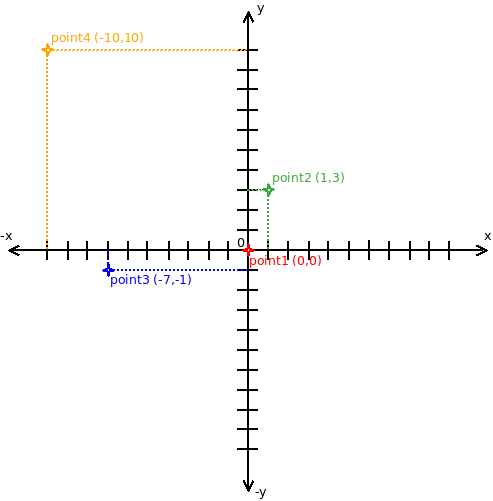
\includegraphics[scale=.6]{monde.png}
 \end{center}
 \caption{Repère orthonormé (monde) avec quelques points (entités mobiles)}
\end{figure}

\vspace{1pt}

\begin{figure}[!h]
 \begin{center}
  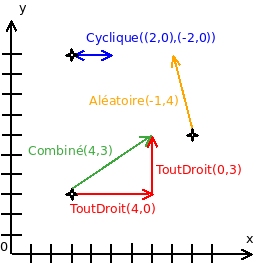
\includegraphics[scale=.6]{mouvements.png}
 \end{center}
 \caption{Quelques vecteurs du plan (mouvements) avec comportements}
\end{figure}

\clearpage

\section*{Détails sur la conception}

Dans ce monde à deux dimensions, on sait qu'il existe plusieurs comportements de déplacement pour les entités mobiles. En matière de conception, le design pattern « Strategy » s'avère alors particulièrement utile car il va nous permettre de choisir un certain comportement à l'exécution. Ici, il convient par conséquent de définir une interface (Comportement) imposant la redéfinition d'une méthode getProchainMouvement() à toutes les classes « comportementales » qui l'implémentent. Conformément au pattern « Strategy », qui va tirer parti du polymorphisme et du liage dynamique, c'est cette méthode qui va contenir toute l'intelligence du programme, ou autrement dit l'algorithme à exécuter en fonction des cas. À ce titre, si on appelle par exemple la méthode getProchainMouvement() sur une entité mobile possédant un comportement « ToutDroit », on s'attend à ce que ce soit la méthode getProchainMouvement() de la classe « ToutDroit » qui soit exécutée, et que bien sûr l'entité aille indéfiniment dans la même direction... Dans la plupart des cas, getProchainMouvement() est d'ailleurs une « factory method » qui renvoie une instance de Mouvement.
D'un point de vue conceptuel, on peut alors dire ici que l'interface Comportement, les classes qui l'implémentent, mais aussi la classe Mouvement induite, constituent une stratégie de comportement. Dans le développement du projet, on a donc pris soin de créer un package « strategie » pour regrouper tout cela.

En dehors de la stratégie pure, qui est en soi le c\oe ur du programme, on a généralement un contexte qui va utiliser cette stratégie (cela a d'ailleurs fait l'objet d'un autre package afin de bien structurer le code). En l'occurrence, ce sont les entités mobiles qui vont utiliser une stratégie de comportement ; entités mobiles qui sont elles-mêmes gérées par le monde. En UML, on a donc une relation d'association entre la classe EntiteMobile et l'interface Comportement. En revanche, la relation de composition semble plus pertinente entre la classe Monde et la classe EntiteMobile. On peut dire en effet que le monde est composé d'entités mobiles et que ces entités mobiles n'ont de raison d'exister que parce qu'il y a un monde. Si le monde est détruit, les entités mobiles doivent l'être également. On sait par ailleurs, comme nous l'avons vu précédemment, qu'une entité mobile n'est pas forcément qu'un simple point dans un plan. Une entité mobile doit donc être abstraite, ça ne peut être qu'un modèle pour d'autres classes. Dans le cadre de cet exercice, nous utilisons exclusivement des points car un point est une représentation simple d'une entité mobile dans un plan (la classe Point étant dérivée de la classe EntiteMobile). Mais on pourrait très bien utiliser un personnage de jeu vidéo en 2D en guise d'entité mobile...

Enfin, on sait désormais que le monde gère ses entités mobiles et que c'est lui qui lance les itérations responsables des différents déplacements. Cette notion d'itération inhérente au monde rendait l'utilisation d'un Iterator particulièrement intéressante. Mais dans notre cas, nous avons utilisé un Iterator déguisé via la boucle « for each » qui possède une syntaxe plus claire et concise que l'Iterator explicite. Nous n'avions d'ailleurs besoin que des méthodes implicites « hasNext » et « next » pour parcourir le monde. Nul besoin d'un « remove » ici.

\begin{landscape}
  \begin{figure}
  \begin{center}
    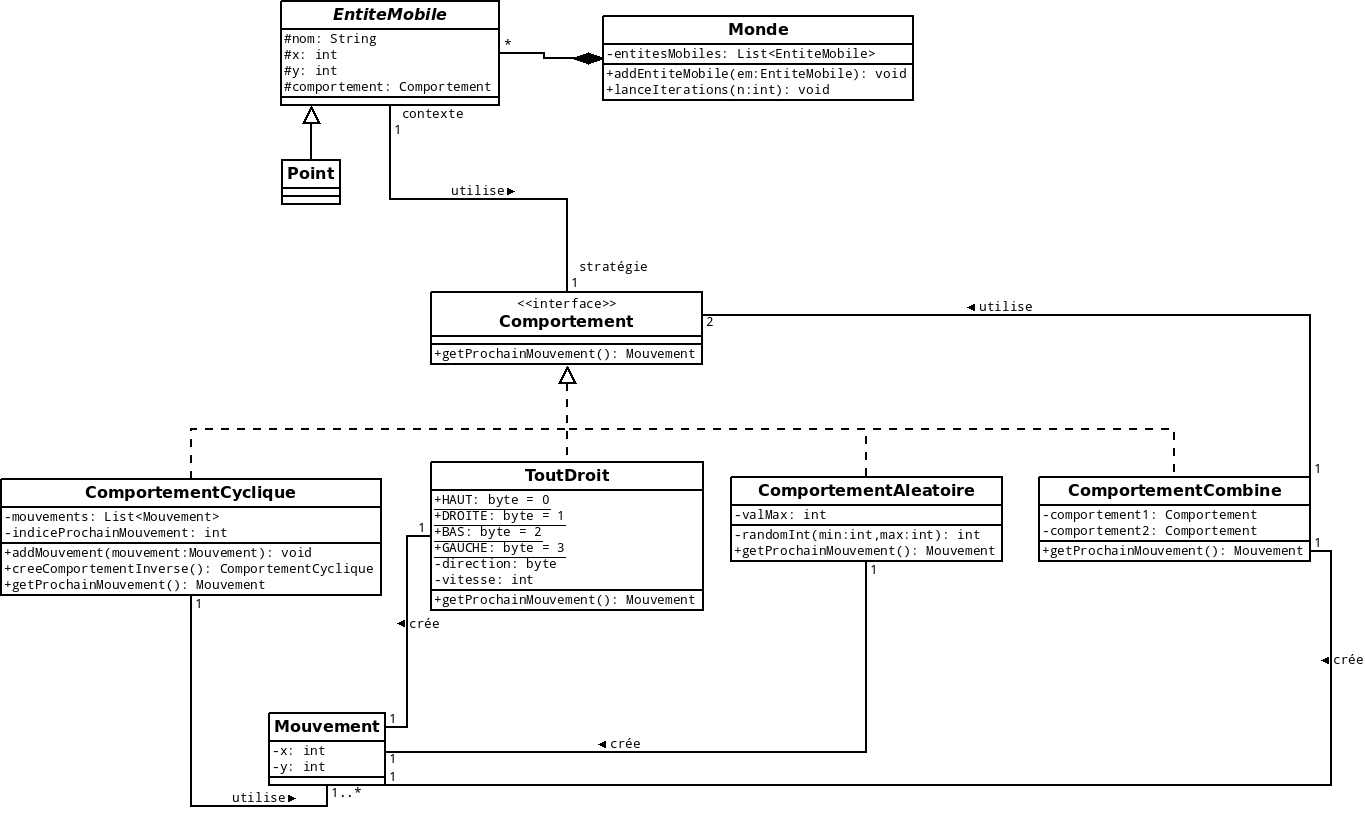
\includegraphics[scale=.4]{entitesMobiles.png}
  \end{center}
  \caption{Diagramme de classes (UML)}
  \end{figure}
\end{landscape}

\textbf{Attention} : les constructeurs, les accesseurs et les mutateurs n'apparaissent pas, volontairement, dans le diagramme UML à des fins de simplification. Ils n'apporteraient pas grand-chose dans la représentation du problème et ne feraient qu'alourdir inutilement le diagramme.

\section*{Détails sur le développement}

Lors du développement, une attention particulière a été portée à la maintenabilité du code, que ce soit en termes de lisibilité ou de performance. À ce titre, et en plus d'avoir une documentation abondante, le code est agencé selon une structure stricte et tente d'éviter au maximum la redondance.

On remarquera que la plupart des classes du projet possèdent deux constructeurs selon le mécanisme de surcharge, dont un par défaut sans paramètres, et l'autre avec tous les paramètres permettant d'initialiser les attributs. Ici, bien sûr, on ne réécrit jamais deux fois la même chose et on utilise systématiquement le « this() » pour éviter le copier-coller.

Dans cette logique d'optimisation, et en gardant à l'esprit la notion de coût inévitable en informatique, les types simples (notamment numériques) ont été choisis avec soin pour ne pas encombrer inutilement la mémoire. Par exemple, pour les constantes de la classe ToutDroit (représentant les quatre directions possibles), il était vraisemblablement intéressant d'utiliser le type byte sur un octet plutôt que le type int sur quatre octets qu'on utilise un peu par réflexe.

Naturellement, certaines opérations représentent un coût important qu'il faut bien accepter : évoquons notamment la double boucle dans la méthode « lanceIterations », où l'on parcourt plusieurs fois d'affilée une ArrayList dans son intégralité. Ces opérations n'ont pas un coût neutre, loin de là, et ce coût peut suivre une progression exponentielle en fonction des besoins du « client~» et du nombre d'entités mobiles constitutives du monde. On peut aussi évoquer les recopies en profondeur au sein du comportement cyclique qui représentent un vrai travail de fond pour le compilateur puisqu'il faut à chaque fois réserver un nombre de cases non négligeable en mémoire (pour une ArrayList) et remplir ces cases avec des objets provenant d'une autre ArrayList qu'il faut bien sûr parcourir... L'ArrayList est néanmoins à sa place dans cet exercice car nous nous contentons globalement d'ajouter des éléments en fin de liste, que ce soit des entités mobiles ou des mouvements, et nous n'avons pas recours à la méthode « remove » qui est pour le moins gourmande en termes de complexité (temps de parcours + décalage de toutes les cases...).

Enfin, on remarquera que le principe d'encapsulation a été systématiquement respecté, bien qu'il s'agisse là d'un travail personnel dont le code ne sera vraisemblablement pas manipulé par un tiers (ce qui limite quand même grandement les mauvais usages qu'on pourrait faire des classes...).

\end{document}
